\documentclass[UTF-8,twoside,cs4size]{ctexart}
\usepackage[dvipsnames]{xcolor}
\usepackage{amsmath}
\usepackage{amssymb}
\usepackage{geometry}
\usepackage{setspace}
\usepackage{xeCJK}
\usepackage{ulem}
\usepackage{pstricks}
\usepackage{pstricks-add}
\usepackage{bm}
\usepackage{mathtools}
\usepackage{breqn}
\usepackage{mathrsfs}
\usepackage{esint}
\usepackage{textcomp}
\usepackage{upgreek}
\usepackage{pifont}
\usepackage{tikz}
\usepackage{circuitikz}
\usepackage{caption}
\usepackage{tabularx}
\usepackage{array}
\usepackage{pgfplots}
\usepackage{multirow}
\usepackage{pgfplotstable}
\usepackage{mhchem}

\newcolumntype{Y}{>{\centering\arraybackslash}X}
\geometry{a4paper,centering,top=0.75cm,bottom=2.54cm,left=2cm,right=2cm}
\pagestyle{plain}
\captionsetup{font=small}

%\CTEXsetup[name={,.}]{section}
\CTEXsetup[format={\raggedright\bfseries\noindent\zihao{3}}]{section}
\CTEXsetup[format={\raggedright\bfseries\quad\large}]{subsection}
\CTEXsetup[format={\raggedright\bfseries\qquad}]{subsubsection}
\renewcommand\thefootnote{\ding{\numexpr171+\value{footnote}}}

\setstretch{1.5}

\setCJKfamilyfont{boldsong}[AutoFakeBold = {2.17}]{SimSun}
\newcommand*{\boldsong}{\CJKfamily{boldsong}}
%\DeclareMathOperator\dif{d\!}
\newcommand*{\me}{\mathop{}\!\mathrm{e}}
\newcommand*{\mpar}{\mathop{}\!\partial}
\newcommand*{\dif}{\mathop{}\!\mathrm{d}}
\newcommand*{\tab}{\indent}
\newcommand*{\mcelsius}{\mathop{}\!{^\circ}\mathrm{C}}

\begin{document}
	\begin{flushright}
		\zihao{2}{分组号:3-07}
	\end{flushright}
	
	\noindent{\zihao{-2}\boldsong\bfseries 《\,\, 基\,\, 础\,\, 物\,\, 理\,\, 实\,\, 验\,\, 》\,\, 实\,\, 验\,\, 报\,\, 告\,\, }
	
	\noindent\textit{实验名称\uline{\quad\qquad\qquad\quad\quad 温度与热导率的测量\,\qquad\qquad\qquad\qquad}指导教师\uline{\qquad\,\,\,张一楠\,\,\,\qquad}}
	
	\noindent\textit{姓\qquad 名\uline{\,\,\, 桂庭辉\,\,\,}\,学号\uline{\,\,\,{\upshape2019K8009929019}\,\,\,}\,专\qquad 业\uline{\,\,\,计算机科学与技术\,\,\,}\,班级\uline{\,\,\,\upshape{03}\,\,\,}\,座号\uline{\,\,\,\upshape{6}\,\,\,}}
	
	\noindent\textit{实验日期\uline{\,\,{\upshape 2020}\,\,}年\uline{\,\,{\upshape 12}\,\,}月\uline{\,\,{\upshape16}\,\,}日\,\,实验地点\uline{\,\,\,教学楼{\upshape427}\,\,\,}调课/补课\uline{\,\,\,$ \square $是\,\,\,}成绩评定\uline{\,\,\,\quad\qquad\qquad}}
	
	\begin{table}[h]
		\centering
		\psset{linewidth=2pt}
		\begin{pspicture}(-1,-0.1)(1,0.1)
		\psline(-9,0)(9,0)
		\end{pspicture}
	\end{table}

	\begin{center}
		\Large\heiti 第一部分\quad 动态法测定良导体的热导率
	\end{center}
	
	\section{实验目的}
	1.通过实验学会一种测量热导率的方法;
	
	2.了解动态法的特点和优越性;
	
	3.认识热波,加强对波动理论的理解。
	
	\section{实验仪器与用具}
	仪器主机由绝热材料紧裹侧表面的圆棒状样品\footnote{本实验选用铜、铝两种样品。}、热电偶列阵、实现边界条件的脉动热源及冷却装置组成。样品中热量将只沿轴向传播,在任意一个垂直于棒轴的截面上各点温度相同。那么只要测得轴线上各点温度分布,就能够确定整个棒体上的温度分布。温度的测量通过热电偶列阵实现:将热电偶偶端均匀插在棒内轴线处,两个相邻偶间距离均为2\,cm,此外还需用冷却水冷却,以保证棒尾的温度$ T_0 $恒定,进而防止整个棒温起伏。
	
	本实验仪器包括样品单元、控制单元和记录单元三大部分,有手动、程控两种工作方式。这两种方式的差异在于记录单元。手动方式使用高精度$ x-y $记录仪,而程控方式用计算机实现对整个系统的控制、数据的采集、记录与绘图。
	
	\section{实验原理}
	在样品上取一小段作为棒元,示意图如图(\ref{difx})。根据热传导定律,单位时间内流过某垂直于传播方向上面积$ A $的热量,即热流为
	\[\frac{\dif q}{\dif t}=-kA\frac{\dif T}{\dif x}\]
	其中$ k $为待测材料热导率,$ A $为截面积,$ \frac{\dif T}{\dif x} $为温度对$ x $的梯度。
	
	\begin{figure}[!h]
		\centering
		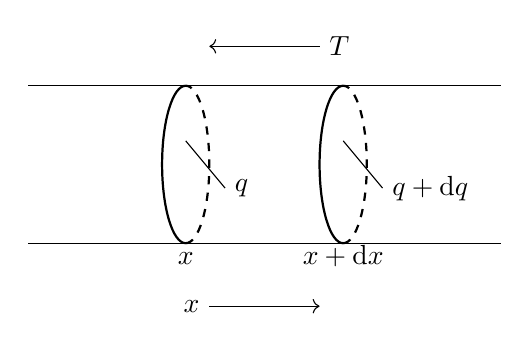
\begin{tikzpicture}
			\draw (0,0)--(6,0);
			\draw (0,2)--(6,2);
			\draw [thick] (2,2) arc (90:270:0.3 and 1);
			\draw [thick, dashed] (2,0) arc (-90:90:0.3 and 1);
			\draw [thick] (4,2) arc (90:270:0.3 and 1);
			\draw [thick, dashed] (4,0) arc (-90:90:0.3 and 1);
			\draw [<-] (2.3,2.5)--(3.7,2.5) node[right]{$ T $};
			\draw [->] (2.3,-0.8) node[left]{$ x $}--(3.7,-0.8);
			\node [below] at(2,0) {$ x $};
			\node [below] at(4,0.1) {$ x+\dif x $};
			\draw (2,1.3)--(2.5,0.7) node[right]{$ q $};
			\draw (4,1.3)--(4.5,0.7) node[right]{$ q+\dif q $};
		\end{tikzpicture}
		\caption{棒元示意图}
		\label{difx}
	\end{figure}

	将上式两边对坐标取微分有
	\[\frac{\dif^2 q}{\dif x\dif t}=-kA\frac{\dif^2 T}{\dif x^2}\,\Longrightarrow\,\dif\frac{\dif q}{\dif t}=-kA\frac{\dif^2 T}{\dif x^2}\]
	
	根据能量守恒定律,任一时刻棒元的热平衡方程为
	\[C\rho A\dif x\frac{\dif T}{\dif t}=\dif\frac{\dif q}{\dif t}=-kA\frac{\dif^2 T}{\dif x^2}\dif x\]
	其中$ C,\,\rho $分别为材料的比热容与密度,由此可得热流方程
	\[\frac{\dif T}{\dif t}=D\frac{\dif^2 T}{\dif x^2}\]
	其中$ D=\frac{k}{C\rho} $称为热扩散系数。上式的解表示了各点温度随时间的变化,其具体形式取决于边界条件。若令热端温度随时间简谐变化,即
	\[T=T_0+T_m\sin\omega t\]
	另一端用冷水冷却,保持恒定低温$ T_0 $,则上式的解,即棒中各点的温度为
	\[T=T_0-\alpha x+T_m\exp\left(-\sqrt{\frac{\omega}{2D}}x\right)\sin\left(\omega t-\sqrt{\frac{\omega}{2D}}x\right)\]
	其中$ T_0 $为直流成分,$ \alpha $为线性成分的斜率,从上式可以看出:
	
	{\kaishu (a)热端$ (x=0) $处温度按简谐方式变化时,这种变化将以衰减波的形式在棒内向冷端传播,称为热波;}
	
	{\kaishu (b)热波波速$ v=\sqrt{2D\omega} $;}	
	{\kaishu (c)热波波长$ \lambda=2\pi\sqrt{\frac{2D}{\omega}} $.}
	
	因此在热端温度变化的角频率已知的情况下,只要测出波速或波长即可计算出$ D $。再由$ D=\frac{k}{C\rho} $计算出材料的热导率$ k $。本实验根据$ v=\sqrt{2D\omega} $可得
	\[v^2=2\frac{k}{C\rho}\omega\,\Longrightarrow\,k=\frac{v^2C\rho}{4\pi f}=\frac{v^2C\rho}{4\pi}T\]
	其中$ f,\,T $分别为热端温度按简谐变化的频率和周期。实现上述测量的关键在于热量在样品中一维传播、热端温度按简谐变化。
	
	\section{实验内容}
	1.检查各处连接管路是否有堵塞,然后打开水源,从出水口观察流量,要求水流稳定。两个冷却水管在两个样品中是串联的,水流先铝后铜,故而一般先测铜样品,后测铝样品,以免冷却水变热。
	
	2.打开电源,主机进入工作状态。
	
	3.打开操作软件,在控制软件中设置热源周期$ T=180\,\mathrm s $,先选用铜样品进行测量。
	
	4.按下“操作”栏中“测量”按钮,使仪器开始测量工作,在窗口上画出$ T-t $曲线族。测量约40分钟后,系统进入动态平衡,样品内温度动态稳定。此时按下“暂停”,在“文件”菜单中保存相应数据。
	
	5.换用铝样品重做步骤4。
	
	6.将实验数据通过网络发送给自己,先关闭测量仪器,再关闭计算机。
	
	\section{实验结果与数据处理}
	相邻热电偶的间距$ l_0=2\,\mathrm{cm} $,周期$ T=180\,\mathrm{s} $,铜的比热为$ 0.385\,\mathrm{J/(g\cdot K)} $,密度为$ 8.92\,\mathrm{g/cm^3} $;铝的比热为$ 0.880\,\mathrm{J/(g\cdot K)} $,密度为$ 2.7\,\mathrm{g/cm^3} $。
	\subsection{动态法测铜的热导率}
	根据记录得到的实验数据\footnote{由于靠后位置的温度变化不明显,仅选取前六个测量位置数据。}可作出如下图像:
	\begin{figure}[!h]
		\centering	
		\begin{tikzpicture}		
			\begin{axis}[
				width=14cm,height=6cm,
%				title={},
				xlabel=$ t\;(\mathrm{s}) $,
				ylabel=信号强度(mV),
				xmin=700,xmax=1700,
				ymin=800,ymax=1400,
				xtick={700,900,1100,1300,1500,1700},
				ytick={800,1000,1200,1400},
				grid style=dashed,
%				ymajorgrids=true,
%				xmajorgrids=true,
				]
				\addplot[red,thick,smooth,no marks] file {Cu-1.txt};
				\addplot[Green,thick,smooth,no marks] file {Cu-2.txt};
				\addplot[blue,thick,smooth,no marks] file {Cu-3.txt};
				\addplot[red,thick,smooth,no marks] file {Cu-4.txt};
				\addplot[Green,thick,smooth,no marks] file {Cu-5.txt};
				\addplot[blue,thick,smooth,no marks] file {Cu-6.txt};
%				\addplot[red,thick,smooth,no marks] file {Cu-7.txt};
%				\addplot[Green,thick,smooth,no marks] file {Cu-8.txt};
			\end{axis}
		\end{tikzpicture}
		\captionsetup{skip=0pt}
		\caption{动态法测铜的热导率数据记录}
	\end{figure}
	
	从原始数据可读到、计算得到如下数据:
	\begin{table}[!h]
		\centering
		\renewcommand\arraystretch{1.5}
		~\
		
		\caption{动态法测铜的热导率数据记录}
		
		\begin{tabularx}{\textwidth}{|c|Y|Y|Y|Y|Y|Y|}
			\hline
			测量点$ n $&0\,cm&2\,cm&4\,cm&6\,cm&8\,cm&10\,cm\\
			\hline
			对应峰值时间$ t(\mathrm s) $&1180.52&1186.04&1193.52&1201.52&1209.52&1220.04\\
			\hline
			波速(m/s)&0.00362&0.00267&0.00250&0.00250&0.00190&—\\
			\hline
		\end{tabularx}
	\end{table}
	
	~\
	
	那么波速的平均值为
	\[\bar V = 0.00264\,\mathrm{m/s}\]
	
	根据公式$ k=\frac{V^2C\rho}{4\pi f}=\frac{V^2C\rho T}{4\pi} $可求得铜的热导率为
	\[k_{\mathrm{Cu}}=\frac{V^2C\rho T}{4\pi}=348.43\,\mathrm{W/(m\cdot\mcelsius)}\]
	\subsection{动态法测铝的热导率}
	\begin{figure}[!h]
		\centering	
		\begin{tikzpicture}		
			\begin{axis}[
				width=14cm,height=7cm,
				%				title={},
				xlabel=$ t\;(\mathrm{s}) $,
				ylabel=信号强度(mV),
				xmin=1400,xmax=2600,
				ymin=700,ymax=1500,
				xtick={1400,1600,1800,2000,2200,2400,2600},
				ytick={700,900,1100,1300,1500},
				grid style=dashed,
				%				ymajorgrids=true,
				%				xmajorgrids=true,
				]
				\addplot[red,thick,smooth,no marks] file {Al-1.txt};
				\addplot[Green,thick,smooth,no marks] file {Al-2.txt};
				\addplot[blue,thick,smooth,no marks] file {Al-3.txt};
				\addplot[red,thick,smooth,no marks] file {Al-4.txt};
				\addplot[Green,thick,smooth,no marks] file {Al-5.txt};
				\addplot[blue,thick,smooth,no marks] file {Al-6.txt};
				%				\addplot[red,thick,smooth,no marks] file {Cu-7.txt};
				%				\addplot[Green,thick,smooth,no marks] file {Cu-8.txt};
			\end{axis}
		\end{tikzpicture}
		\captionsetup{skip=0pt}
		\caption{动态法测铝的热导率数据记录}
	\end{figure}
	
	由上图易见第五个测量点起始部分数据有误,故选取峰值时间应选用$ t=2000\,\mathrm s $附近的峰值数据,而非首个峰值点。
	
	\begin{table}[!h]
	\centering
	\renewcommand\arraystretch{1.5}
	\caption{动态法测铝的热导率数据记录}
	\begin{tabularx}{\textwidth}{|c|Y|Y|Y|Y|Y|Y|}
		\hline
		测量点$ n $&0\,cm&2\,cm&4\,cm&6\,cm&8\,cm&10\,cm\\
		\hline
		对应峰值时间$ t(\mathrm s) $&1900.52&1905.52&1913.04&1923.04&1933.52&1941.52\\
		\hline
		波速(m/s)&0.00400&0.00266&0.00200&0.00191&0.00250&—\\
		\hline
	\end{tabularx}
	\end{table}
	那么波速的平均值为
	\(\bar V=0.00261\,\mathrm{m/s}\),
	所以可求得铝的热导率为
	\[k_{\mathrm{Al}}=\frac{V^2C\rho T}{4\pi}=231.84\,\mathrm{m/s}\]
	
	\newpage
	
	~\
	
	\begin{center}
		\Large\heiti 第二部分\quad 温度的测量和温度计的设计
	\end{center}
	\setcounter{section}{0}
	
	\section{实验目的}
	1.用电位差计测热电偶的温差电动势;
	
	2.用平衡电桥测热敏电阻和铜电阻的温度特性曲线;
	
	3.设计非平衡电桥实现对热敏电阻的实时测量。
	
	\section{实验仪器与用具}
	\subsection{DHT-2热学实验装置温控仪}
	本实验采用DHT-2型热学实验仪进行温度计的控温,其内装有热电偶温度计、铜电阻温度计、热敏电阻温度计,通过加热丝升温、风扇降温,可以用来测试不同类型温度计的温度特性曲线、确定温度系数等。
	
	使用过程中依次将“信号输入”、“加热电流”依次与加热炉上接口相连,然后连接电源、打开电源开关。
	
	按设定键(S)选择温度位数,用上下键加减数值,连续未按设定键(S)八秒,自动停止闪烁并返回正常显示设定值。设定加热温度后打开面板上的加热电流开关。本次实验中建议加热电流为$ 0.6\,\mathrm A $。
	\subsection{UJ36a型携带式直流电位差计}
	本实验采用UJ36a型携带式直流电位差计测量热电偶的电压。利用补偿法原理测量直流电压(或电动势)和对各种直流毫伏表及电子电位差计进行刻度矫正。
	
	本次实验的实际调节过程中,接入待测电压后将倍率开关拨到“$ \times 0.2 $”,调零检流计,将电键开关拨到“标准”,调节工作电流调节变阻器,使检流计再次指零,将电键开关拨到未知。调节滑线读数盘使得检流计再次置零,那么未知电压读数为
	\[U_x=\text{滑线盘读数}\times\text{倍率}\]
	\subsection{DHQJ-5型教学用多功能电桥}
	本实验采用DHQJ-5型教学用多功能电桥进行电阻测定与温度计的实时测量,具有开放式电桥、双臂电桥、单臂电桥、功率电桥和非平衡使用的单臂电桥等功能,本次实验主要再单臂电桥下,用平衡电桥测温度计的电阻,用非平衡电桥对温度计进行实时测量。
	
	在平衡电桥下,检流计中的电流与电压均为0,则待测电阻值为
	\[R_x=\frac{R_2}{R_1}R_3\]
	
	非平衡电桥是单臂电桥在非平衡状态下的一种工程应用。DHQJ-5在非平衡使用时,其造作步骤基本与单臂电桥相同,但测量目的与方法有很大差异,在本次实验中,选用非平衡电桥电压的变化线性表示热敏电阻温度计测量温度的变化。
	
	\section{实验原理}
	\subsection{用电位差计测热电偶的温差电动势}
	热电偶又被称作温差电偶,是由A,B两种不同材料的金属丝的端点彼此紧密接触而成的。当两个接点处于不同温度$ t,\,t_0 $时,在回路中会产生直流电动势,该电动势被称为温差电动势或热电动势。当组成热电偶的材料一定时,温差电动势$ E_x $仅与两接点处的温度有关,且两接点的温度在一定温度范围内有如下近似关系式:
	\[E_x\approx\alpha(t-t_0)\]
	其中$ \alpha $称为温差电系数,对于不同金属组成的热电偶,$ \alpha $不同。%其数值上等于两接点温度差为1\,\textcelsius 时产生的电动势。
	
	为了测量温差电动势,就需要将热电偶接入电位差计,但测量仪器的引入不能影响热电偶的性质,故而实验时需保证一定条件。根据伏打定律,即在A,B两种金属之间接入第三种金属C,且其与A,B两接点处于同一温度,这样的闭合回路的温差电动势与上述只有A,B两种金属组成回路中的温差电动势数值完全相同。所以通常将A,B两根化学成分不同的金属丝一端焊接在一起,构成热电偶的热端,将另两端各与铜引线\footnote{即第三种金属C。}焊接,构成两个同温度的冷端。
	
	铜引线与电位差计相连,从而构成了一个热电偶温度计。通常将冷端置于冰水混合物中,保持$ t_0=0 $\,\textcelsius,将热端置于待测温度处,即可测得相应的温差电动势。%再根据事先校正好的曲线或数据来求出温度$ t $。
	
%	热电偶温度计有点在于热容量小、灵敏度高、反应迅速、测温范围广,还能将温度转换成电学量,因此其再自动测温、控温等系统中得到广泛应用。
	
	\subsection{用平衡电桥测电阻的温度特性曲线}
	\subsubsection{金属电阻温度计}
	一般而言,金属电阻随温度的变化规律为
	\[R_x=R_{x0}(1+\alpha t+\beta t^2)\]
	其中$ R_{x0} $为$ t=0 $\,\textcelsius 时的电阻值。如铜电阻的相关参数为
	\[R_{x0}=50\,\Omega\qquad \alpha=4.289\times10^{-3}\mcelsius^{-1}\qquad \beta=2.133\times10^{-7}\mcelsius^{-2}\]
	
	通常,在温度不是很高的情况下,可忽略温度二次项$ \beta t^2 $,从而可将金属的电阻值随温度的变化看作线性变化,即
	\[R_x=R_{x0}(1+\alpha t)=R_{x0}+\alpha tR_{x0}\]
	利用控温仪将铜电阻的温度控制在一系列的温度值上,待温度稳定后,用平衡电桥测出铜电阻的阻值,画出温度--阻值曲线,进行线性拟合即可求出温度系数。
	
	\subsubsection{半导体热敏温度计}
	半导体热敏电阻NTC通常由一些金属氧化物如$ \mathrm{Fe_3O_4} $、$ \mathrm{MgCr_2O_4} $等半导体制成。在这些半导体内部,自由电子数目随着温度升高迅速增加,导电能力的增强很快,所以NTC具有负的电阻温度系数,随着温度升高,其电阻值迅速下降。通过改良也可以设计出正温度系数的热敏电阻,简称PTC。
	
	热敏电阻的电阻温度特性可以用下述指数函数来描述:
	\[R_T=A\me^{B/T}\]
	式中$ A $是与材料性质的电阻器几何形状有关的常数,$ B $是与材料半导体性质有关的常数,$ T $为绝对温度。
	
	为了求得准确的$ A,B $,可将上式两边取对数:
	\begin{equation}\label{2-3-2-2-1}
		\ln R_T=\ln A+\frac BT
	\end{equation}
	选定不同的温度$ T $,可得到不同的$ R_T $。
	
	当$ T=T_1 $时,有
	\[\ln R_{T_1}=\ln A+\frac{B}{T_1}\]
	当$ T=T_2 $时,有
	\[\ln R_{T_2}=\ln A+\frac{B}{T_2}\]
	将以上两式相减后可得
	\begin{equation}\label{2-3-2-2-2}
		B=\frac{\ln R_{T_1}-\ln R_{T_2}}{\frac{1}{T_1}-\frac{1}{T_2}}
	\end{equation}
	常用半导体热敏电阻的$ B $值约在$ 1500\sim 5000\,\mathrm K $之间。

	将式(\ref{2-3-2-2-2})代入式(\ref{2-3-2-2-1})可得
	\begin{equation}\label{2-3-2-2-3}
		A=R_{T_1}\me^{-B/T_1}
	\end{equation}
	
	利用控温仪将热敏电阻温度控制在一系列温度点上,用平衡电桥测出相应的电阻,根据式(\ref{2-3-2-2-1})进行线性拟合,可以求出热敏电阻的温度系数$ A,\,B $;若只测两个温度点,也可以通过式(\ref{2-3-2-2-2}),(\ref{2-3-2-2-3})求出$ A,\,B $.
	
	\subsection{设计非平衡电桥实现对热敏电阻的实时测量}
	非平衡电桥的电路图如下图所示:
	\begin{figure}[!h]
		\centering
		\begin{circuitikz}
			\draw (0.8,0.5)
			to[short] (0,0)
			to[short,o-] (-2.5,0)
			to[short] (-2.5,3)
			to[short,-*] (-2,3)
			to[european resistor,-*,l={$ R_1 $},a={$ I_1 $}] (0,4.5)
			to[european resistor,-*,l={$ R_3 $},a={$ I_3 $}] (2,3);
			\draw (-2,3)
			to[european resistor,-*,l={$ R_2 $},a={$ I_2 $}] (0,1.5)
			to[european resistor,-*,l={$ R_x $},a={$ I_4 $}] (2,3);
			\draw (0,4.5)
			to[short] (0,5)
			to[short] (3,5)
			to[voltmeter,l={$ U_0 $}] (5,5)
			to[short] (5,1)
			to[short] (0,1)
			to[short] (0,1.5);
			\draw (0.9,0)
			to[battery,o-,a={$ E $}] (3,0)
			to[short] (3,3)
			to[short] (2,3);
			\node[below] at(0.45,0) {$ K $};
		\end{circuitikz}
		\caption{非平衡电桥电路图}
	\end{figure}
	
	非平衡电桥的测试步骤与平衡电桥一样,只是选用电压表测两端电压,认为电压表内阻无穷大,忽略流过电压表的电流。平衡时电桥电压为0,而非平衡电桥电压$ U_0 $随$ R_x $实时变化,通过计算选取合适的$ R_1,\,R_2,\,R_2 $以及$ E $,让测试电压$ U_0 $随温度$ t $线性变化,则可以对温度进行实时测量。
	
	可求得
	\begin{equation}\label{2-3-3-1}
		U_0=\left(\frac{R_x}{R_2+R_x}-\frac{R_3}{R_1+R_3}\right)E
	\end{equation}
	其中
	\begin{equation}\label{2-3-3-2}
		R_x=A\me^{B/T}
	\end{equation}
	$ A,B $的值可分别根据式(\ref{2-3-2-2-2}),(\ref{2-3-2-2-3})求得。
	
	将式(\ref{2-3-3-2})代入式(\ref{2-3-3-1})即可得到$ U_0 $与$ T $间的函数关系,对$ U_0 $作泰勒展开,略去三阶及以上的高阶项,可以得到
	\[U_0=U_{01}+U_0'(T-T_1)+U_0''(T-T_1)^2\]
	其中$ T_1 $为测试区间的中间值,例如监测$ 30\sim 50 $\,\textcelsius 的温度区间,取$ T_1=40\mcelsius $。令$ U_0''=0 $,可得
	\begin{equation}\label{28}
		R_x=A\me^{B/T}=\frac{B+2T}{B-2T}R_2
	\end{equation}
	那么得到$ U_0 $关于$ T $的线性表达:
	\[U_0=\lambda+m(t-t_1)\]
	其中
	\[\lambda=\left(\frac{B+2T_1}{2B}-\frac{R_3}{R_1+R_3}\right)E=U_{01},\quad m=\left(\frac{4T_1^2-B^2}{4BT_1^2}\right)E=U_0'\]
	由于是温度差,绝对温度$ T $可换成摄氏温度$ t $。而$ \lambda $表示在温度区间中间值时对应的$ U_0 $值,$ m $表示灵敏度。
	
	根据选定的$ \lambda,\,m $,由两个温度点求得$ A,\,B $,以及式(\ref{28})可计算得到$ R_2,\frac{R_1}{R_3},E $,具体表达式如下:
	\[E=\left(\frac{4BT_1^2}{4T_1^2-B^2}\right)m,\quad R_2=\frac{B-2T}{B+2T}R_{xT_1},\quad\frac{R_1}{R_3}=\frac{2BE}{(B+2T_1)E-2B\lambda}-1\]
	根据计算结果即可设定非平衡电桥的相应参数。
	
	\section{实验内容}
	\subsection{用电位差计测热电偶的温差电动势}
	1.在室温下测得热电偶的电动势。
	
	2.开启温控仪电源,对热端加热,在$ 30\sim 50\mcelsius $区间内每隔$ 5\,\mcelsius $测定一组$ (t,E_x) $\footnote{需等温度稳定后进行读数测量。}。
	
	3.绘制温度特性曲线,通过线性拟合求得温度系数。
	\subsection{用平衡电桥测热敏电阻和铜电阻的电阻值}
	1.在室温下测得热敏电阻、铜电阻的电阻值。
	
	2.在$ 30\sim 50\,\mcelsius $区间内每隔$ 5\mcelsius $测定一组$ (t,R_x) $。
	
	3.绘制温度特性曲线,通过线性拟合求温度系数。
	\subsection{用非平衡电桥制作热敏电阻温度计}
	选定$ \lambda = -400\,\mathrm{mV},\; m=-10\,\mathrm{mV/\mcelsius},\; t_1=40\mcelsius $,根据在$ 30\mcelsius,\;50\mcelsius $下测得的热敏电阻大小计算$ A,\,B $,进而计算$ E,\,R_2,\,\frac{R_1}{R_3} $.
	
	根据计算结果设定非平衡电桥的参数,将温控仪温度设定为$ 40\mcelsius $,微调$ R_2 $阻值,使得电压表测得电压接近$ -400\,\mathrm{mV} $。
	
	改变温控仪温度,在$ 40\sim 50\mcelsius $区间内,每隔$ 2.5\mcelsius $测得一组$ U_0,\,t $,观察自制温度计测温的精度。
	
	\section{实验结果与数据处理}
	
	\subsection{用电位差计测热电偶温差电动势}
	实验时置冷端于冰水混合物中,即保持冷端温度为$ 0\mcelsius $,在室温$ t=21.9\mcelsius $下测得电动势$ E_x=0.640\,\mathrm{mV} $。
	
	调整温度,实验数据记录如下:
	
	\begin{table}[!h]
		\centering
		\renewcommand\arraystretch{1.5}
		\caption{不同温度下热电偶的温差电动势}
		\begin{tabularx}{\textwidth}{|c|Y|Y|Y|Y|Y|}
			\hline
			温度$ t\,(\mcelsius) $&30.0&35.3&40.3&44.9&50.2\\
			\hline
			电动势$ E_x\,(\mathrm{mV}) $&0.998&1.192&1.404&1.592&1.790\\
			\hline
		\end{tabularx}
	\end{table}
	
	根据上表数据可作出如下拟合图象:
	
	\begin{figure}[!h]
		\centering
		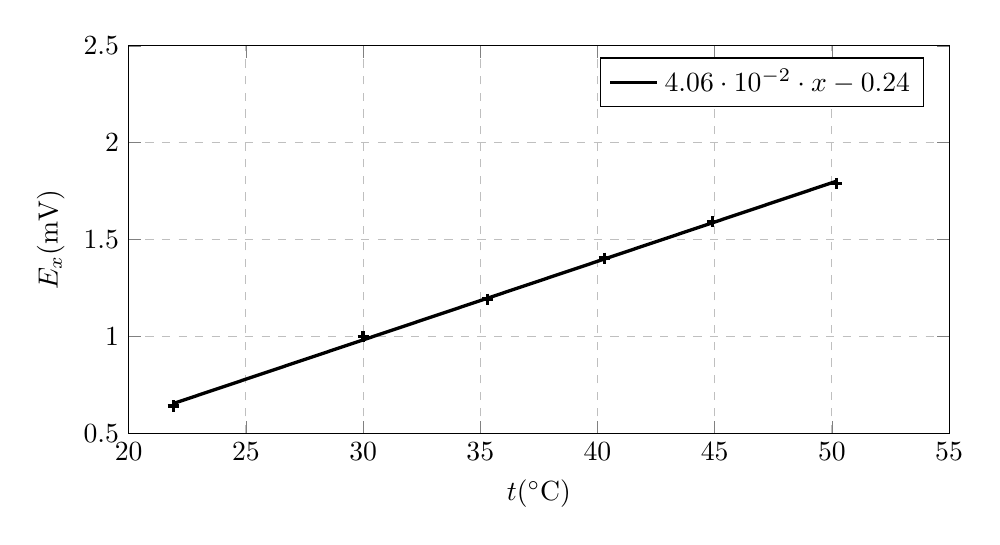
\begin{tikzpicture}
			\begin{axis}[
				legend pos=north east,
				width=12cm,height=6.5cm,
				xlabel=$ t(\mcelsius) $,
				ylabel=$ E_x(\mathrm{mV}) $,
				xmin=20,xmax=55,
				ymin=0.5,ymax=2.5,
				xtick={20,25,30,35,40,45,50,55},
				ytick={0.5,1,1.5,2,2.5},
				grid style=dashed,
				ymajorgrids=true,
				xmajorgrids=true,
				]
				\addplot[no marks,black,very thick] table[y={create col/linear regression={y=Y}}]
				{
					X	Y
					21.9	0.640
					30	0.998
					35.3	1.192
					40.3	1.404
					44.9	1.592
					50.2	1.790			
				};
				\addlegendentry{
					$\pgfmathprintnumber{\pgfplotstableregressiona} \cdot x
					\pgfmathprintnumber[print sign]{\pgfplotstableregressionb}$}
				
				\addplot [very thick,mark=+,only marks] coordinates {
					(21.9,0.640)(30,0.998)(35.3,1.192)(40.3,1.404)(44.9,1.592)(50.2,1.790)
				};
			\end{axis}
		\end{tikzpicture}
		\caption{热电偶温差电动势与温度间关系}
	\end{figure}
	
	由式$ E_x\approx\alpha(t-t_0) $可知上述拟合直线的斜率即为热电偶的温差电系数
	\[\alpha = 0.0406\,\mathrm{mV/\mcelsius}\]
	
	\subsection{平衡电桥测铜电阻温度特性曲线}
	在室温$ t=21.5\mcelsius $下测得铜电阻阻值为$ R_x=56.7\,\Omega $。
	
	调整温度,实验数据记录如下:
	\begin{table}[!h]
		\centering
		\renewcommand\arraystretch{1.5}
		\caption{不同温度下铜电阻阻值}
		\begin{tabularx}{\textwidth}{|c|Y|Y|Y|Y|Y|}
			\hline
			温度$ t\,(\mcelsius) $&30.0&35.3&40.3&44.9&50.2\\
			\hline
			电阻$ R_x\,(\Omega) $&58.6&59.7&61.1&62.2&63.3\\
			\hline
		\end{tabularx}
	\end{table}
	
	根据上表数据可作出如下拟合直线:
	\begin{figure}[!h]
		\centering
		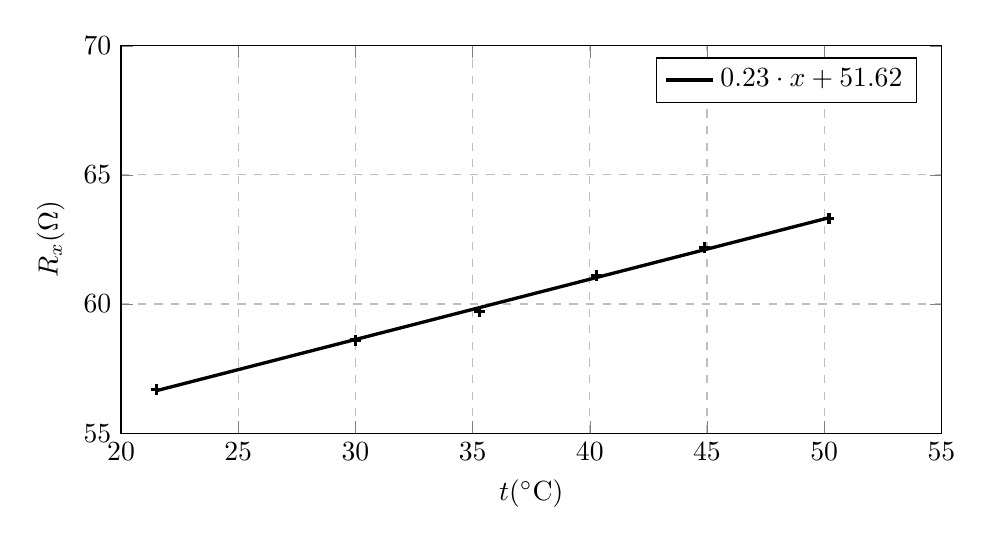
\begin{tikzpicture}
			\begin{axis}[
				legend pos=north east,
				width=12cm,height=6.5cm,
				xlabel=$ t(\mcelsius) $,
				ylabel=$ R_x(\Omega) $,
				xmin=20,xmax=55,
				ymin=55,ymax=70,
				xtick={20,25,30,35,40,45,50,55},
				ytick={55,60,65,70},
				grid style=dashed,
				ymajorgrids=true,
				xmajorgrids=true,
				]
				\addplot[no marks,black,very thick] table[y={create col/linear regression={y=Y}}]
				{
					X	Y
					21.5	56.7
					30.0	58.6
					35.3	59.7
					40.3	61.1
					44.9	62.2
					50.2	63.3			
				};
				\addlegendentry{
					$\pgfmathprintnumber{\pgfplotstableregressiona} \cdot x
					\pgfmathprintnumber[print sign]{\pgfplotstableregressionb}$}
				
				\addplot [very thick,mark=+,only marks] coordinates {
					(21.5,56.7)(30,58.6)(35.3,59.7)(40.3,61.1)(44.9,62.2)(50.2,63.3)
				};
			\end{axis}
		\end{tikzpicture}
		\caption{铜电阻阻值与温度间关系}
	\end{figure}
	
	由公式$ R_x=R_{x0}+\alpha tR_{x0} $可知
	\[R_{x0}=51.62\,\Omega,\quad \alpha=\frac{0.23}{51.62}\mcelsius^{-1}=0.0045\mcelsius^{-1}\]
	
	\subsection{平衡电桥测热敏电阻温度特性曲线}
	在室温$ t=21.4\mcelsius $下测得热敏电阻阻值为$ R_T=2806.5\,\Omega $,则$ \ln R_T=7.939 $.
	
	改变温度,记录数据如下:
	\begin{table}[!h]
		\centering
		\renewcommand\arraystretch{1.5}
		\caption{不同温度下热敏电阻阻值}
		\begin{tabularx}{\textwidth}{|c|Y|Y|Y|Y|Y|}
			\hline
			温度$ t\,(\mcelsius) $&30.0&35.3&40.3&44.9&50.2\\
			\hline
			$ \frac1T\,(\mathrm K^{-1}) $&0.00330&0.00324&0.00320&0.00314&0.00309\\
			\hline
			电阻$ R_T\,(\Omega) $&1937.4&1597.5&1306.7&1082.5&894.8\\
			\hline
			$ \ln R_T $&7.564&7.376&7.175&6.987&6.797\\
			\hline
		\end{tabularx}
	\end{table}

	根据上表数据可作出$ \ln R_T-\frac1T $图象如下页。
	
	\begin{figure}[!h]
		\centering
		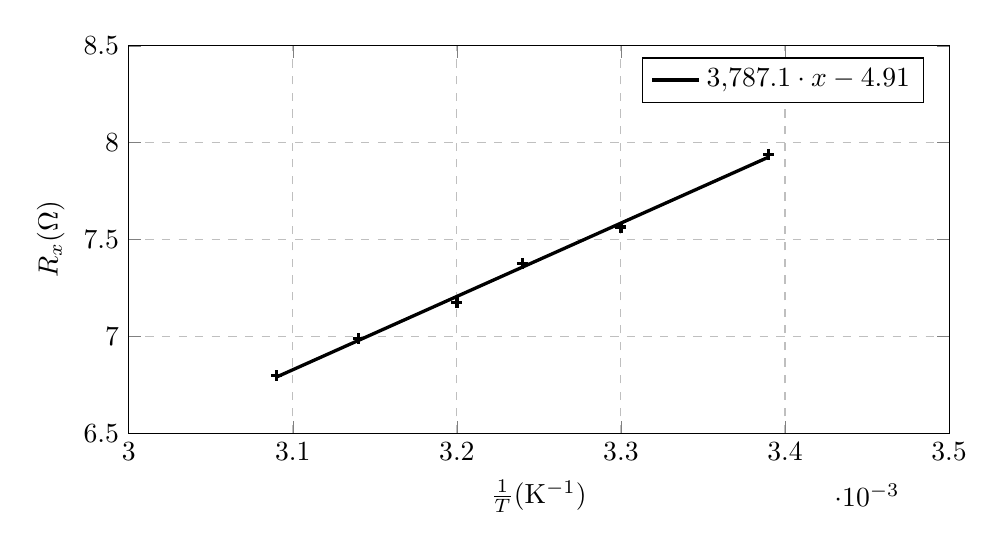
\begin{tikzpicture}
			\begin{axis}[
				legend pos=north east,
				width=12cm,height=6.5cm,
				xlabel=$ \frac1T(\mathrm K^{-1}) $,
				ylabel=$ R_x(\Omega) $,
				xmin=0.003,xmax=0.0035,
				ymin=6.5,ymax=8.5,
				xtick={0.003,0.0031,0.0032,0.0033,0.0034,0.0035},
				ytick={6.5,7,7.5,8,8.5},
				grid style=dashed,
				ymajorgrids=true,
				xmajorgrids=true,
				]
				\addplot[no marks,black,very thick] table[y={create col/linear regression={y=Y}}]
				{
					X	Y
					0.00339	7.939
					0.00330	7.564
					0.00324	7.376
					0.00320	7.175
					0.00314	6.987
					0.00309	6.797	
				};
				\addlegendentry{
					$\pgfmathprintnumber{\pgfplotstableregressiona} \cdot x
					\pgfmathprintnumber[print sign]{\pgfplotstableregressionb}$}
				
				\addplot [very thick,mark=+,only marks] coordinates {					
					(0.00339,7.939)
					(0.00330,7.564)
					(0.00324,7.376)
					(0.00320,7.175)
					(0.00314,6.987)
					(0.00309,6.797)
				};
			\end{axis}
		\end{tikzpicture}
		\caption{$ \ln R_T-\frac1T $拟合直线}
	\end{figure}

	根据公式$ \ln R_T=\ln A+\frac BT $可知
	\[B=3787.1,\quad A=0.00737\]
	
	\subsection{非平衡电桥热敏电阻温度计的设计}
	温度区间:$ 30\sim 50\mcelsius $
	
	热敏电阻特性常数:$ A=0.00731,\;B=3786.9 $\footnote{此处计算所用数据不包含室温下的数据,故与上小节结果不同。}
	
	表头参数选择:$ \lambda=-0.4\,\mathrm V,\;m=-0.01\,\mathrm{V/\mcelsius} $
	
	工作电源电压:$ E=1.0660\,\mathrm V,\;R_2=936.7\mcelsius,\;\frac{R_1}{R_3}=0.0439 $
	
	实际值:$ R_2=945.6\,\Omega,\;R_1=43.9\,\Omega,\;R_3=1000\,\Omega $
	
	热敏电阻温度计测试温度$ t(\mcelsius) $与测试电压$ U_0 $的关系为
	\[U_0=\lambda+m(t-t_1)\,\Longrightarrow\,t=\frac{U_0-\lambda}{m}+t_1\]
	调整温度应用该温度计测试温度的结果如下:
	\begin{table}[!h]
		\centering
		\renewcommand\arraystretch{1.5}
		\caption{热敏电阻温度计的测试}
		\begin{tabularx}{\textwidth}{|c|Y|Y|Y|Y|Y|}
			\hline
			设定温度$ t\,(\mcelsius) $&39.9&42.5&45.0&47.5&50.0\\
			\hline
			测试电压$ U_0\,(\mathrm{mV}) $&-400&-426&-451&-477&-502\\
			\hline
			测试温度$ (\mcelsius) $&40.0&42.6&45.1&47.7&50.2\\
			\hline
		\end{tabularx}
	\end{table}

	\newpage
	
	~\
	
	\begin{center}
		\Large\heiti 第三部分\quad 思考题与实验总结
	\end{center}
	\setcounter{section}{0}
	
	\section{思考题}
	1.如果想知道某一时刻$ t $时材料棒上的热波,即$ T-x $曲线,将如何做?
	
	{\kaishu 在该时刻下,以各测量点的位置坐标为横坐标,各测量点的热电偶测量数据为纵坐标作图。若想得到效果更好的$ T-x $图象,则需使用更为密集的热电偶阵列。}
	
	~\
	
	2.为什么较后面测量点的$ T-t $曲线振幅越来越小?
	
	{\kaishu 在热波从近端向远端传播时,由于热阻的存在有一部分能量损失,从而使得热波的振幅随着$ x $的增大而减小,故而靠后的测量点上的$ T-t $曲线振幅逐渐减小。}
	
	~\
	
	3.为什么实验中铝棒的测温点才8个,而铜棒的测温点达到12个?
	
	{\kaishu 铝棒的热导率与铜相比较小,故而曲线振幅下降得较快,在8个测量点后$ T-t $曲线的振幅过小不易观察,不利于数据采集与热导率计算。而热导率较高的铜则在12个测量点后才会出现这样的问题。}
	
	~\
	
	4.实验中误差的来源有哪些?
	
	{\kaishu 实验误差可能来自:(1)实际使用的样品棒具有一定粗细,平行于截面的热波传播影响了实验数据。(2)实验器材带来的误差,如热电偶质量、传感器间距、水流稳定程度、热电偶灵敏度等。(3)数据处理过程中峰值的选取策略带来的误差。}
	
	~\
	
	5.为什么在低温实验中常用四线式伏安法测温度,而工业仪表中常用非平衡电桥测温度?
	
	{\kaishu 低温实验对电路精度的要求很高,而待测电阻值通常较低。四线式伏安法能消除导线电阻对电路带来的误差影响,以高精度测得较低电阻值,符合低温实验的要求。}
	
	{\kaishu 工业上对精度没有实验中那么高的要求,在保证效果的情况下通常会选用更为经济、易用的方式。而非平衡电桥更为经济,在输出、控制等方面上比四线式更为灵活,故而能在工业上得到较为广泛的应用。}
	
	~\
	
	6.工业仪表中使用的三线式非平衡电桥测温度是怎么消除引线电阻的?
	
	{\kaishu 三线式非平衡电桥的电路示意图见下页。当电桥两臂上的引线电阻(即为$ R_1,\,R_2 $所在支路)大致相等时,引线电阻对于实验结果的影响相互抵消,从而消除了引线电阻的影响。}
	
	~\
	
	\begin{figure}[!h]
		\centering
		\begin{circuitikz}
			\draw (0,0)
			to[battery,l=$ E $] (0,4)
			to[short] (2,4)
			to[european resistor,a=$ R_1 $,*-*] (2,2)
			to[european resistor,a=$ R_2 $,-*] (2,0)
			to[short] (0,0);
			\draw (2,4)
			to[european resistor,l=$ r_1 $] (8,4)
			to[european resistor,l=$ R_x $,-*] (8,2)
			to[short](8,0);
			\draw (2,2)
			to[voltmeter,l=$ U_{\text{out}} $] (5,2)
			to[european resistor,l=$ r_2 $] (8,2);
			\draw (2,0)
			to[variable european resistor,l=$ R_{\text{p}} $] (5,0)
			to[european resistor,l=$ r_3 $] (8,0);
		\end{circuitikz}
		\caption{三线式平衡电桥示意图}
	\end{figure}
	\section{实验总结}
	在本次实验中,除了对热学知识有了进一步的了解外,还体会了计算机、自动化在物理实验中的应用、半导体的应用、电磁学在热学实验中的应用。虽然实验器材或有损耗,但这也促使我在数据处理上慎之又慎,力求精确。
\end{document}